\chapter{System Design}

\section{Framework Selection}

\subsection{LeapMotion \& LeapJS}

% LeapMotion \ cite {Leap: 2016} is a general term for a hardware input device and its software,
% Its hardware built two depth camera and an infrared detector can detect the hand within the field of view,
% Part of its software with built-in model for the detection of bone re-modeling of the hand, and then complete the behavior of high-precision hand
% \ Footnote {LeapMotion claims official recognition accuracy of 0.01mm,
% Document \ cite {weichert2013analysis, gdu2016} analysis showed LeapMotion actual accuracy of 0.2 mm or so. }
% Recognition.
LeapMotion \cite{Leap:2016} is a general term for a hardware input device and its software, its hardware built by two depth camera and an infrared detector that can detect the hand within the field of view; its software built-in a skeleton model of hands for hand reconstruct\footnote{ LeapMotion's official accuracy is 0.01 mm, but \cite{weichert2013analysis, gdu2016} report its actural accuracy is 0.2 mm}.
%LeapMotion \cite{Leap:2016}是一个硬件输入设备和其自身软件的一个总称,
%其硬件中内置的两颗深度摄像头和一个红外探测器可以对视野内的手检测,
%其软件部分利用内置的骨骼模型对检测的手部进行重新建模,进而完成手行为的高精度
%\footnote{ LeapMotion 的官方宣称的识别精度为 0.01mm,
%文献\cite{weichert2013analysis, gdu2016} 分析表明 LeapMotion 的实际精度在 0.2 mm 左右。}
%识别。
LeapMotion SKD provides two varieties of API for getting the LeapMotion data: a native interface and a WebSocket interface, WebSocket provides JavaScript interface in browser environment. It is conforms to RFC6455\footnote{\url{http://tools.ietf.org/html/rfc6455}}, and running on desktop default port 6437.
%LeapMotion SDK 有两种风格的 API 可以用于获取 LeapMotion 提供的手部数据:
%本地接口及 WebSocket 接口,WebSocket 接口便其提供了浏览器环境中的 JavaScipt 接口。
%LeapMotion 的 WebSocket 服务遵循 RFC6455
%\footnote{\url{http://tools.ietf.org/html/rfc6455}},
%运行在连接 LeapMotion 硬件的桌面端的 6437 端口。

LeapJS is the JavaScript framework for LeapMotion Controller.
Using LeapJS enables Web font-end communication with LeapMotion, and this framework is used for processing LeapMotion JSON data.
With NodeJS, LeapJS also can running on server side, thus we can also processing LeapMotion interaction on server side by JavaScript.
%而 LeapJS 就是 LeapMotion 控制器的客户端 JavaScript 框架。
%使用 LeapJS 可以让 LeapMotion 与网页前端进行通信,此框架可以用来处理接受 LeapMotion JSON 消息。
%但随着 NodeJS 的存在,LeapJS 也能够运行在服务端,
%因此我们也能够在服务端使用 JavaScript 处理 LeapMotion 消息。
Leap API gives a Frame object, which contains a Hand object if the hand of users can be detected in LeapMotion field of view. LeapMotion through its buit-in model of hands, reconstruct hands object and then provide its to developers.
for example, it provides hand direction, hand finger direction, hand position in LeapMotion coordinate system.
%Leap API 以 Frame 为对象,当可被检测的手出现在 LeapMotion 视野内时,
%深度摄像头捕捉到的每个 Frame 都能够访问到一个 Hand 对象。
%Leap 通过对手部的重新建模,将当前帧的手部信息提供给开发者,
%例如当前手的指向、当前手在 LeapMotion 坐标系统下的位置。
With LeapMotion, developer and researcher can avoid the basic image segement works and other stuff, them keep focus on gesture algorithm\cite{garber2013gestural,xusuibin2015,panjiajia2015,huhong2015,marin2014hand}.
%借助 LeapMotion 能够省去开发者的手部检测和识别的部分基础工作,更多的关注于手势算法的研究\cite{garber2013gestural,xusuibin2015,panjiajia2015,huhong2015,marin2014hand}。

In addition, 3D gesture already gains its application in simple method, \cite{zaicti2015free} gives a LeapMotion control interaction for TV.
%另外,空间手势已经得到较成熟简单应用,例如文\cite{zaicti2015free}基于 LeapMotion 实现了 TV 上的控制。

\subsection{watchOS \& WatchConnectivity}

watchOS is the operating system that runs on the Apple Watch. When watchOS just released, applications only as an extension for iOS App, watchOS only illustrate annimations, all code runs on iOS.
%watchOS 是运行在 Apple Watch 上的操作系统。watchOS 刚推出时,
%第三方 App 是作为 iOS 的应用扩展存在,手表端只负责对代码的执行结果进行展示,所有的代码都在 iOS 端执行。

With lunching of watchOS 2, now applications can use WatchConnectivity framework to pass data between iOS and watchOS.
%随着 watchOS 2 的发布,现在第三方 App 能够通过 WatchConnectivity 框架在 watchOS 和 iOS 之间进行数据通信。

WatchConnectivity framework aims to makes message between iOS and watchOS to be a message in system level, developer shouldn't care much about it. These communication will start a seesion and only WCSession.defaultSession.reachable is true, the dilivery can be started. So if we would use WatchConnectivity, we must implement WCSessionDelegate protocol.
%使用 WatchConnectivity 框架执行的通信必须经过 watchOS 和 iOS 系统级的中转。这些通信在 iOS 端和 watchOS 端开启一个会话,因此若需要使用 WatchConnectivity,就必须要实现 WCSessionDelegate 代理协议。

Besides, WatchConnectivity contains two differnt communication module: backgroung module and interactive module. In backgroung module, OS will push the message into a queue, then process it when App wake up; In interactive module, message must trasfer through OS and it is an immedientely communication, only happens when WCSession.defaultSession().reachable is true.

It is worth mentioning that, in interactive module, even if the iOS client program has not yet started, the Apple Watch is still able to wake up an iOS App from background.
%另外,在 WatchConnectivity 中存在两种不同的通信模式:后台模式和交互式消息模式。在后台模式中,操作系统会将一些非及时消息发送到等待消息队列,并在 App 被唤醒时进行处理;而在交互是消息模式中,由于通信必须经过系统级的中转,因此 watchOS 和 iOS 之间的及时通信,仅当检查到 WCSession.defaultSession().reachable 为真时,才能够进行通信。值得一提的时,在交互式消息中,即便 iOS 端程序尚未启动,在 Apple Watch 中依然能够从后台将 iOS 应用唤醒。

\section{Architecture}
\label{sec:arch-design}

\subsection{Communication Structure}
\label{sub:im-arch}

watchOS splited from iOS App Extension since 2.0 version, since then, watchOS can actrully excute code on Apple Watch, that make watchOS App can management communication\cite{WatchGuide:2016} between iOS App and itself, the structure as illustrate on \ref{fig:watch-phone}. This makes timely communication with the outside world be possible.
%watchOS 从 2.0 开始从 iOS App Extension 中剥离开来,将 Watch App 部分全部移至 watchOS 端,
%这时这部分代码在手表端具备了可执行的权限,因此将 watchOS 从 1.0 中的单向接收 iOS 端的系统级的通信,
%转变为第三方 App 执行管理\cite{WatchGuide:2016},如图 \ref{fig:watch-phone} 所示。
%这使其与外界的及时通信成为了可能。

\begin{figure}[H]
    \kaishu
    \centering
    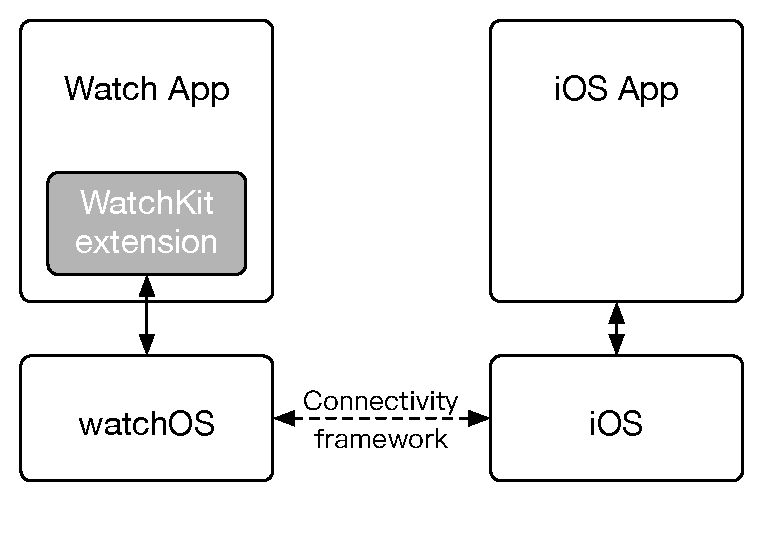
\includegraphics[width=0.4\textwidth]{figures/watch-phone}
    \caption{\kaishu Connection between Watch App, WatchKit Extension and iOS App}
    \label{fig:watch-phone}
\end{figure}

However, there are still load of limits for networking on watchOS. In watchOS 2, Apple Watch only when its paired iPhone disconnected and its also in a saved WiFi environment that can access internet by using NSURLSession, these conditions are rigor.
%然而,即便如此在 watchOS 上的网络访问能力依然十分有限,在 watchOS 2 中,
%Apple Watch 只能在和与其配对的 iPhone 失去连接,且同时处于已保存的 Wi-Fi 网络覆盖范围内时,才能独立使用 NSURLSession 访问网络,条件十分苛刻。

In consideration of above, we designed the communication architecture and illustrate it on Figure \ref{fig:im-arch}.
%鉴于以上考虑,本文对从服务端到客户端的通信架构设计如图 \ref{fig:im-arch} 所示。

\begin{figure}[H]
    \kaishu
    \centering
    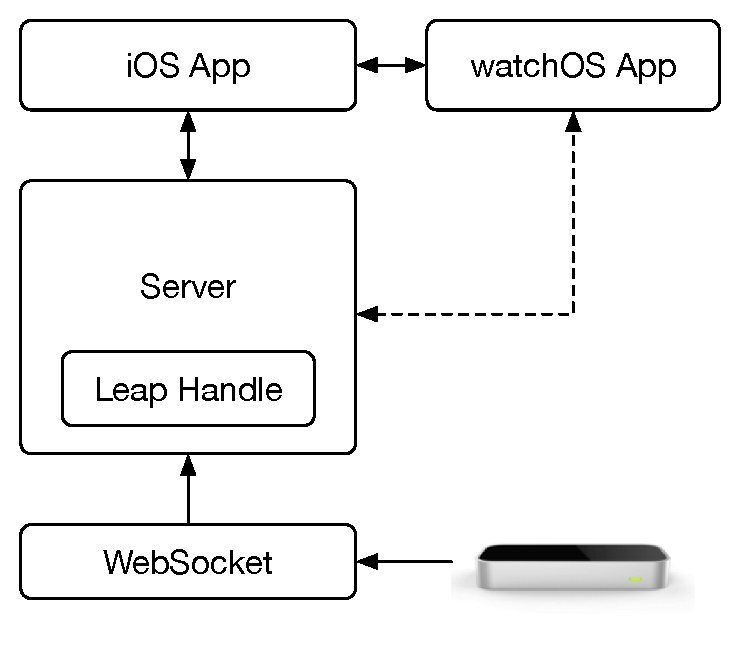
\includegraphics[width=0.4\textwidth]{figures/arch}
    \caption{\kaishu \textbf{Communication Architecture}: iOS App as a router to transfer message between watchOS and server, instead of watchOS directly communicate to server}
    \label{fig:im-arch}
\end{figure}

Among this architecture, iOS App will be the bridge for watchOS App and server for processing interaction message, watchOS only cares content present.
%其中,watchOS 将 iOS 端作为与服务器通信的桥梁,处理性能及其有限的 watchOS 端仅负责对通信内容的呈献,
%性能稍强的 iOS 端对服务端消息进行筛选与加工,而服务端则对 LeapMotion 原始数据进行分析,
%并封装其分析结果后与 iOS 端进行通信。

\subsection{Client Structure}

Client side includes iOS side and watchOS side, as shows on \ref{fig:client-arch}.
%客户端包含 iOS 端和 watchOS 端两个部分,其架构设计如图 \ref{fig:client-arch} 所示。

\begin{figure}[H]
    \kaishu
    \centering
    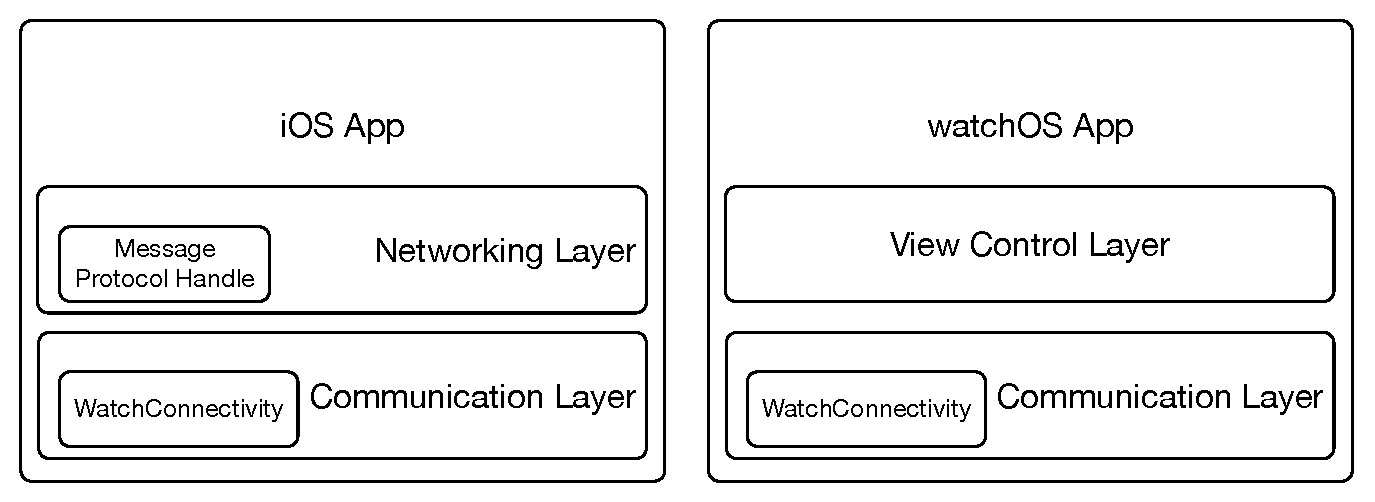
\includegraphics[width=0.6\textwidth]{figures/client-arch}
    \caption{\kaishu \textbf{Client side structure}: iOS App process server message then send the results to communication layer to watchOS, watchOS react the interaction manipulate UI elements by view controller layer when it recived the message.}
    \label{fig:client-arch}
\end{figure}

\subsection{Server Structure}

Server side structure as its shown on Figure \ref{fig:server-arch}, the core mocule is Interaction Handle Layer, this layer process raw interaction data from sensors and post the interaction results to Request Handle layer then distribute it to suitable devices.
%服务端的设计如图 \ref{fig:server-arch} 所示,其组件的核心是交互处理层,
%该层负责对原始的交互数据进行加工处理为将要实施的交互消息,
%然后将加工后的消息按消息协议封装好进而通过请求层分发给相应的请求对象。

\begin{figure}[H]
    \kaishu
    \centering
    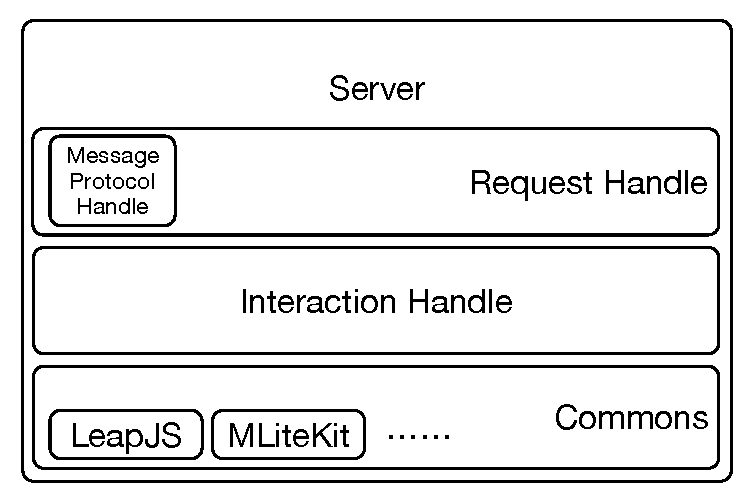
\includegraphics[width=0.4\textwidth]{figures/server-arch}
    \caption{\kaishu \textbf{Server side structure}: Interaction Handle Layer process raw interaction data, then post it to Request Handle Layer for data tranfer}
    \label{fig:server-arch}
\end{figure}

\section{Communication Protocol}

We need design the interaction message communication protocol between watchOS, iOS and server.
%我们需要设计在 watchOS 和 iOS 之间、iOS 与 服务端之间设计相关的交互通信协议。

According to Figure \ref{fig:interaction}, basic interaction gesture contains grab, two fingers swipe and tree different tap(thumb with index, middle, ring finger), the two fingers means thumb and index finger.
%根据图\ref{fig:interaction}所示,用户与手表端进行交互时共涉及五指合并、双指滑动、手指点击三个基本操作,
%其中双指滑动仅指拇指和食指之间的滑动。而对于交互本身的表达,
%在图\ref{fig:im-arch}中被设计为由 iOS 端进行表达。

For this reason, interaction message field design as in Table \ref{table:server-feild}.
%因此,对于服务端与 iOS 端之间的通信数据字段设计如下:

\begin{table}[H]
    %\scriptsize
    \small
    \kaishu
    \centering
    \setlength{\belowcaptionskip}{10pt}
    \caption{Interaction Protocol Fields}
    \begin{tabular}{c l l}
        \toprule
        \textbf{Field}        & \textbf{Type} & \textbf{Description} \\
        \hline
        pinchTimeStramp & Date  & Time of pinch operate\\
        pinchIndex     & int    & Finger index of pinch, from 1 to 4 express index finger to little finger, -1 means no finger \\
        pinchStrength  & double & Strength of pinch, from 0 to 1, real number \\
        grabStrength   & double & Grab strength, from 0 to 1, real number \\
        forceValue     & double & Simulate value of Force Touch\\
        \bottomrule
    \end{tabular}

    \label{table:server-feild}
\end{table}

\section{Demonstrate Programs}

Although we conducted a comprehensive interactive design, but due to the restriction on the development of Apple Watch, we are unable to operate the view in system-level. In this thesis, we gives five alternative interactive demos with different effects.
%尽管我们对交互方式进行了完备的设计,但由于 Apple Watch 开发上的限制,我们无法对系统级的视图进行操作,因此本文对备择交互一共给出了以下的五个不同效果的演示。

\begin{itemize}
    \kaishu
    \item Demo 1: This demo shows the alternative interaction design of tap gesture;
    %第一个演示程序展示了手表点按交互的备择交互设计方案,如图所示;
    \item Demo 2: This demo shows the alternative interaction design of swipe gesture;
    %第二个演示程序展示了手指在手表屏幕上滑动的备择交互设计方案,如图所示;
    \item Demo 3: This demo shows the alternative interaction design of Digital Crown;
    %第三个演示程序展示了对 Apple Watch 所特有的 Digital Crown 的备择交互设计,如图所示;
    \item Demo 4: This demo shows the alternative interaction design of Force Touch;
    %第四个演示程序展示了对 Apple Watch 所特有的 Force Touch 的备择交互设计方案,如图所示;
    \item Demo 5: This demo illustrate a contact-free game experiences on Apple Watch.
    %第五个演示程序展示了一个非接触式交互的游戏案例。
\end{itemize}

Above five demos video can be found in YouTube
%以上五个演示程序的演示视频可以在 YouTube
\footnote{\url{https://www.youtube.com/playlist?list=PLwUqqMt5en7c2QaQ_DkuvZm9dGTz6RjRM}}
, for other related resources, such as source code, see Appendix \ref{appendix:a}.
%链接中查看,项目源码等相关资源及其使用许参见附录\ref{appendix:a}。

\cleardoublepage
